\documentclass[12pt]{article} 

\usepackage{graphicx}
\usepackage[bottom]{footmisc}
\usepackage[utf8]{inputenc} 
\usepackage[T1]{fontenc}
\usepackage[backend=biber, style=numeric]{biblatex}
\usepackage{imakeidx}
\usepackage[toc,page]{appendix}
\usepackage{listings}
\usepackage{xcolor}
\usepackage{pdflscape}
\usepackage{tabularx}
\usepackage{booktabs}
\usepackage{mathpartir}
\usepackage{amsmath}
\usepackage{amssymb}
\usepackage{semantic}
\usepackage{array}
\usepackage{mathtools}
\usepackage{stmaryrd}
\usepackage{longtable}
\DeclareUnicodeCharacter{0308}{\"{}}

\definecolor{codegreen}{rgb}{0,0.6,0}
\definecolor{codegray}{rgb}{0.5,0.5,0.5}
\definecolor{codepurple}{rgb}{0.58,0,0.82}
\definecolor{backcolour}{rgb}{0.95,0.95,0.92}

\newcommand{\grey}[1]{\textcolor{gray}{#1}}
\newcommand{\Q}{\mathcal{Q}}

\lstdefinestyle{mystyle}{
    backgroundcolor=\color{backcolour},   
    commentstyle=\color{codegreen},
    keywordstyle=\color{magenta},
    numberstyle=\tiny\color{codegray},
    stringstyle=\color{codepurple},
    basicstyle=\ttfamily\footnotesize,
    breakatwhitespace=false,         
    breaklines=true,                 
    captionpos=b,                    
    keepspaces=true,                 
    numbers=none,                    
    numbersep=5pt,                  
    showspaces=false,                
    showstringspaces=false,
    showtabs=false,                  
    tabsize=2
}
\lstset{style=mystyle}
\addbibresource{./bibliography/biblio.bib}

% Compile with: pdflatex -shell-escape main.tex
\immediate\write18{texcount -1 -sum -merge \jobname.tex > \jobname.wc}
\newcommand\wordcount{\input{\jobname.wc}}

% -------------------------------
% Metadata
% -------------------------------
\author{K. Chinchilla Flores 1526925 \\ Supervisor: Dr. Christine Rizkallah}
\title{Cedar: Declarative Data Layouts for C} 
\date{2025-11-03}

\begin{document}

% -------------------------------
% Title page
% -------------------------------
\maketitle

\newpage
\section*{Declaration of Authorship}
\addcontentsline{toc}{section}{Declaration of Authorship}
I certify that

\begin{itemize}
    \item This thesis does not incorporate without acknowledgment any material
    previously submitted for a degree or diploma in any university; and that
    to the best of my knowledge and belief it does not contain
    material previously published or written by another person where due
    reference is not made in the text.
    \item No clearance was necessary from the University Ethics committee.
    \item The thesis is \wordcount\ words in length (excluding
    text in images, table, bibliography, and appendices).
\end{itemize}
\\[0.75em]

\newpage
\addcontentsline{toc}{section}{Abstract}
\abstract{
    Cedar is a protoype programming language and compiler that introduces
    declarative byte-level data-layout specication to the C programming
    ecosystem.
    Low-level software such as device drivers, network stacks, and embedded
    systems often require precise control over how data structures are
    represented in memory.
    In the C programming langauge, these details are typically implicit,
    expressed through field ordering, alignment directives, or
    implementation-sepcific pragmas. Such mechanisms are powerful
    but error-prone, and layout inconsistencies are a major source of system
    failures and security vulenerabilities.

    Cedar builds on ideas from Dargent, a verified layout description
    language integrated into the Cogent programming langauge.
    Cedar also borrows from CompCert, the formally verified C compier.
    Rather than pursuing full formal verification, Cedar explores how
    Dargent's declarative approach can be realized directly within
    conventional C development. The language allows programmers to
    specify the structure and placement of data fields using high-level
    constructs such as records, absolute and relative byte offsets,
    endianness annotations, and fixed-length arrayss. Each layout
    is compiled into C code that represents the structure as a flat array
    of 32-bit words, with automatically generated accessor and mutator
    functions for every field.

    The implementation comprises a four-stage pipeline: parsing, lowering,
    checking, and code generation.
    This mirrors the refinement structure of CompCert while remaining small and
    inspectable.
    The prototype supports nested records, per-field endianness, and relative
    or absolute placements, and it generates portable C deo output that has
    been tested to compile succesfully with both GCC and CompCert.
    Evaluation on representative layout examples demonstrate that Cedar can
    express complex C-style structures clearly and that its generated code
    matches the offsets and sizes produced by standard compilers.

    By making layout intent explicit and checkable, Cedar offers a practical
    step towrads trustworthy data-layout specification without imposing a 
    new programming model or sacrificing compatibility with exisiting toolchains.
    The project highlights a path between unverified low-level programming
    and fully verified systems: a middle ground where clarity and correctness
    can coexists with C's performance and flexibility.
}

\newpage
\section*{Acknowledgements}
\addcontentsline{toc}{section}{Acknowledgements}
I would like to express my deepest gratitude to \textbf{Dr. Christine Rizkallah},
my supervisor, for her invaluable guidance, patience, and
encouragement throughout this project. Her insight and feedback
shaped both the technical direction and clarity of this thesis.

I would also like to thank \textbf{George Anderson}, whose
original prototype of Cedar's concept formed the foundation
on which this work was built. His prior contributions mae this
research possible.

Finally, I extend my thanks to \textbf{Vincent Jackson} for his
thoughtful and patient discussions and advice during the
development of this work


% -------------------------------
% Contents (before main text)
% -------------------------------
\newpage
\tableofcontents
\newpage
\listoftables
\newpage
\listoffigures
\newpage

% -------------------------------
% Main text
% -------------------------------
\section{Introduction}

\subsection{Motivation}
Systems programming in C remains foundational to modern computing
infrastructure\autocite{dist_systems_languages, C_embedded_programming}.
Operating systems, hardware drivers, and performance-critical software
all depend on the C language's direct access to
memory\autocite{memory_errors_stridharan}.
Yet the same flexibility that makes C efficient also makes it fragile:
small inconsistencies in layout can cause catastrophic runtime
errors \autocite{evaluation_memory_errors, C_errors_study}.
Layout-related faults—incorrect padding, mis-aligned fields, or unintended
aliasing—manifest as memory corruption and undefined behaviour.
These faults are notoriously difficult to detect, especially when they arise
from hand-crafted structures that must precisely conform to hardware
or protocol formats.

In response, verified programming languages such as
\textbf{Cogent}\autocite{dargent}
have have demonstrated that a functional, type-safe systems code
can be compiled to efficient C with formal correctness guarantees.
However, Cogent and similar languages abstract away and exist in their own
ecosystems. The \textbf{Dargent} framework withing Cogent partly addresses this
issue by allowing the specification of \textit{data layouts} alongside
high-level data types, generating C structs and accessors that obey those
specifications.

Despite its promise, Dargent exposes an inherent challenge: layouts must be
low-level enough to control bits and bytes, yet compositional enough
to reason and verify. Its design is also closely tied to Cogent's compiler,
which makes reuse outside that context difficult. These limitations motiviate
the development of an independent, declarative language for describing and
generating correct low-level layouts—a language that can serve both as a
research vehicle for reasoning about memory representations, and as a
practical tool for C programmers. 

\subsection{Research Aim and Question}
This thesis explores how a small, declarativce language can express complex
memory layouts while preserving reasoning about correctness. The project
defines a prototype langauge, \textbf{Cedar}, originally proposed by
Anderson\autocite{cedar_george}, which treats data layouts as a first-class
concern. Cedar allows programmers to describe how values of structured types
occupy memory, decoupling layout from logical structure.

The central \textbf{research question} guiding this work is:
\begin{quote}
    \textbf{How can the Cedar language be designed and evaluated to support
    practical, verifiable specification of data layouts in C?}
\end{quote}

Answering this question requires both language-design research and
implementation engineering. The goal is not only to reproduce Dargent-style
behaviour in an independent compiler, but also to generalise and clarify
underlying principles: compositional layout descriptions, well-typed accessors,
and generation of C code.

\subsection {Approach and Methodology}
The research follows a \textit{design-and-evaluation} methodology typical
of programming-language research\autocite{incremental_development}.
The work proceeds in three interlocking stages:
\begin{enumerate}
    \item \textbf{Language Design and Formalisation — } analyising the previous
    Cedar proposal and revising its intermediate representations
    (L $\rightarrow$ LR $\rightarrow$ CR) to better capture nexsted records, arrays,
    and bitfields.
    \item \textbf{Implementation and Code Generation — } implementing the Cedar
    compiler to emit cohesive, self-contained C output for representative
    examples, enabling direct comparison with Dargent's generated code.
    \item \textbf{Evaluation via Case Studies — } running the Cedar compiler on
    examples to assess expressivity, correctness, and consistency of generated
    C output.
\end{enumerate}

Throughout these stages, the design is informed by principles from declarative
programming, as it is implemented in a functional style using Haskell.
Rather aiming for a complete verification effort, this thesis focuses
\textit{enabling correctness}: defining interfaces, type rules, and translation
structures that would later support formal reasoning. 
    
\subsection{Contributions}
The main contributions of this thesis are:
\begin{itemize}
    \item \textbf{An extended Language Design for Cedar —} supporting nexsted
    record layouts, bitfields, and more expressive alignment semantics, while
    retaining declarative composition.
    \item \textbf{A Refined Compilation Pipeline —} a modular transofromation
    from surface syntax to layout-resolved forms
    ( L $\rightarrow$ LR $\rightarrow$ CR ) culminating in generated C code that
    preserves structure and alignment.
    \item \textbf{A Prototype Implementation —} a working Cedar compiler
    implemented in Haskell, integrating parsing, type checking layout matching,
    and code generation.
    \item \textbf{Empirical Evaluation via Case Studies —}  reproduction
    of Dargent examples to demonstrate Cedar's usability and internal
    consistency.
    \item \textbf{Discussion of Design Trade-offs and Future Verification
    Pathways —} identifying the boundaries between declarative specification,
    compiler automation, and machine-checkable proof of correctness.
\end{itemize}

Collectively, these outcomes advance Cedar from a concept to a more
complete research language, and contribute new insights into the design of
trustworthy data-layout languages for C.

\subsection{Thesis Structure}
The remainder of this thesis is organised as follows:
\begin{itemize}
    \item \textbf{Chapter 2} reviews background material on C memory layouts,
    verified compilation, the Cogent and Dargent frameworks, and the origins
    of Cedar.
    \item \textbf{Chapter 3} describes the research methodology and language design,
    detailing Cedar's intermediate representations and translation
    pipeline.
    \item \textbf{Chapter 4} presents the implementation and evaluation,
    including case case studies. 
    \item \textbf{Chapter 5} discusses design implications, limitations,
    and directions for future verification and usability improvements.
    \item \textbf{Chapter 6} concludes with a summary of findings and prospects
    for integrating Cedar into broader verified-systems toolchains.
    
\end{itemize}



\section{Background and Related Work}
Low-level systems software depends on correct algorithms but also on
how data is represented in memory. Choices about field order, alignment, and
bit layout can affect performance, portability, and correctness. This chapter
surveys research and industrial work that informs Cedar's design. It begins
with an overview of the problem space, followed by a 
discussion.of C's memory model and layout hazards.
The chapter then examines verified compilers and formal memory 
models, declarative and industrial data-layout
languages,
and runtime analysis tools for detecting memory errors.
The final section synthesizes these threads and
identifies the gap that motivates Cedar's contribution.

\subsection{Overview} \label{5-background}
Precise control over data representation is a defining features of systems
programming. Languages such as C give programmers direct access to memory
through pointers and explicit layout constructs, enabling high-performance
and hardware-proximate code~\autocite{memory_bottleneck, C_embedded_programming}.
At the same time, this flexibility introduces persistent risks: implicit
padding, inconsistent alignment across architectures, and aliasing behaviors
that are only partly defined by the C
standard~\autocite{whatyouc, strict_aliasing}. Even when program logic is
sound, representation errors can lead to subtle faults, security
vulnerabilities, or degraded cache
performance~\autocite{memory_errors_stridharan, C_errors_study, adt_layout_faria}.

Research addressing these challenges has developed along several path.
\textbf{Verified compilation} project such as CompCert and Cogent seek
machine-checked correctness of compiler\
translations~\autocite{leroy2012compcert, cogent1}, but typically assume that
input programs already have well-defined memory layouts.
\textbf{Declarative schema languages} such as PADS, DataScript, and industrial
tools like FlatBuffers or Cap'n Proto make data representation explicit for
serialization, though they operate through generated APIs rather than
arbitrary in-pace C 
structures~\autocite{fisher2005pads,back2002datascript,flat_buffers,capn_proto_serialization}
Meanwhile, \textbf{runtime tools} such as Valgrind and AddressSanitzier detect
invalid memory accesses dynamically, identifyion many errors only after
execution~\autocite{valgrind, asan}.

Cedar builds insights from these areas to explore a \textbf{declarative,
C-oriented approach} to describing layouts directly. The remainder of the chapter
sets out the background required to understand that design: the characteristics
of C's memory model, the verified-compiler lineage, declarative layout
framework and complementary runtime safety tools.

% figure of ambiguous C struct layout showing padding and bit-field packing
%differences

\subsection{The C Memory Model and Layout Challenges}
Systems programming relies on the ability to manipulate data structures
directly in memory. The C language provides this capability by exposing
pointers, address arithmetic, and low-level layout control, allowing
programmers to express data representations to map efficiently
to hardware~\autocite{ritchie1993development, memory_bottleneck}. While
this flexibility enables fine-tuned performance, it also transfers
responsibility for correctness to the programmer. C itself does not enforce
consistent object representations: compilers may vary in how they align, pad,
and order fields, and the standard intentionally leaves these details
under-specified~\autocite{whatyouc,strict_aliasing}.

In practice, these ambiguities lead to \textbf{layout errors} such as
implicit padding, mis-aligned fields, and overlapping bit-fields. all of
which can produce silent data corruption or access errors. For example,
structure layouts may differ across architectures or compilers even when
their source definitions are 
identical~\autocite{packetc_bitfields,compiler_vulns}. The C99 and C11
standards permit compilers to insert padding bytes for alignment, but do not
prescribe how or where these bytes appear. The resulting uncertainty
complicates binary interoperability, particularly for programs that
must communicate through shared memory, files, or hardware registers.

The impact of representation decisions is not limited to correctness. Data
layout strongly influences \textbf{cache locality} and therefore
overall performance~\autocite{adt_layout_faria,kandemir1998enhancing,majeti2013compiler}.
Empirical studies show that reorganizing fields or converting
arrays-of-structures into structures-of-arrays can yield significant
performance gains, underscoring the representation is both a semantic
and performance
concern~\autocite{perry2010automatic}.

To control layout, programmers use mechanisms such as \texttt{struct} for field 
ordering bit-fields and \texttt{union}, often combine with compiler-specific
directives like \texttt{\#pragma pack} or
\texttt{\_\_attribute\_\_((packed))}~\autocite{C_structures}. These features
are essential when implementing device drivers, network stacks, or
file-system components that must match predefined binary
formats~\autocite{network_memory_layouts,device_drivers}. Yet their semantics
are fragile: even small changes in type definitions or compiler options
can alter offsets or alignment unexpectedly. Because the correctness of these
constructs is not checked statically, developers resort to
\textbf{trial-and-error inspection}—printing offsets or using debuggers to
verify field positions—rather than relying on language guarantees.

The consequences of layout mistakes are well documented. Mis-aligned accesses
can crash embedded firmware; incorrect field boundaries in protocol headers
can expose vulnerabilities exploitable through malformed
input~\autocite{memory_errors_stridharan,memory_errors_stridharan}; and
inconsistent packing across architectures breaks cross-platform file or
network formats. Each example reflects a deeper issue: the lack of a formal
abstraction boundary between a type's \textit{semantic structure} and its
\textit{physical representation} in  memory. Without such
boundary, reasoning about correctness or
portability becomes extremely difficult, both for programmers
and for automated analysis tools.

C's weak memory model compounds to this difficulty. The standard defines
memory in terms of abstract "objects" and "effective types", but
optimizations relies on assumptions such as the \textbf{strict aliasing rule}
which are frequently violated in low-level
code~\autocite{strict_aliasing,whatyouc}. These rules can cause
apparently safe pointer casts to yield undefined behavior, particularly in code that
manipulates raw binary data. Formal memory models developed for verified
compilers, such as CompCert's block-and-offset model, explicitly
exclude such cases from their semantics~\autocite{leroy2012compcert}.
As a result, even when C code is verified at a higher level, layout
mismatches or aliasing violations remain outside the verified envelope.

These challenges highlight the need for \textbf{explicit, verifiable layout
specifications}. A language mechanism that clearly separates logical types
from their physical representation could prevent many classes of low-level
bugs, improve portability, and enable reasoning about performance effects.
Later sections of this chapter review verified and declarative approaches that
aim to provide such abstractions. 

% Figure of a steuct whose layout differs in gcc and clang

\subsection{Verified Compilers and Formal Memory Models}
Formal verification has become a central technique for establishing trust
in low-level software systems. Rather than detecting errors through testing,
verified compilers and proof assistants attempt to \textbf{prove
semantic preservation}: that the compiled program behaves exactly as
specified by its source semantics~\autocite{leroy2012compcert}. This
approach has produces verified toolchains such as \textbf{CompCert}, and,
more recently, high-level verified systems languages such as
\textbf{Cogent}~\autocite{cogent1}.

\subsubsection{Verified Compilation and the C Memory Model}
\textbf{CompCert} is a formally verified C to assembly whose proof,
mechanized in Coq, ensures functional equivalence between source and 
target programs under a rigorously defined
model~\autocite{leroy2012compcert,compcert,tolmach2024defining}.
CompCert's \textit{block-and-offset} model treats memory as
a  collection of abstract objects rather than a flat byte array, allowing it
to reason about pointers and aliasing while avoiding undefined behavior. The 
model deliberately abstracts away physical layout: byte order, field alignment,
and padding are not represented. As a consequence, CompCert's correctness
theorem applies only to programs that never depend on the concrete
arrangement of bytes in memory~\autocite{tolmach2024defining}.
Programs that perform bit-level reinterpretation of data or depend on packed
representations fall outside its verified envelope.

This abstraction limits the reach of formal verification for systems
code that must match \textbf{external binary specifications}—for example,
device drivers or network protocol stacks that manipulate precise bit layouts.
Verified compilation ensures that a compiler will not introduce new errors,
but it does not guarantee that a given structure definition correctly
corresponds to its hardware or wire-format specification. Addressing this
gap requires reasoning not just about program behavior, but
about the \textbf{correspondence between logical types and concrete 
memory representations.}

\subsubsection{From Verified Compilers to Verfied Systems Languages}

The \textbf{Cogent} language was developed to make verification of systems
components practical by constraining features and integrating compilation with
theorem-proving~\autocite{cogent1}. Cogent is a \textbf{total, strongly
typed, purely functional language} that compiles to C and simultaneously
generates a formal model in Isabelle/HOL. This dual output allows
refinement proofs showing that the generated C implementation faithfully
realizes the semantics of the Cogent program. Cogent's design enforces
properties such as \textbf{linearity of state} and \textbf{absence of
undefined behavior}, enabling verified systems components like file systems
and kernel modules to be produced.

However, Cogent's abstract data types still required manual, ad-hoc mappings to
the concrete C layouts they referenced. The need to express these mappings
precisely led to the development of \textbf{Dargent}.

\subsubsection{Declarative Layouts in Cogent: The Dargent Extension}
\textbf{Dargent} extends Cogent with a \textbf{declarative language for
specifying data layouts}. Introduced as "Bringing Effortless Refinement
of Data Layouts to Cogent"~\autocite{dargent_isola}, it allows programmers
to define how algebraic data types should be represented at the bit level 
withing memory, elimination much of the manual marshalling previously
required. Layouts are expressed separately from type definitions and are
checked for \textbf{well-formedness}, ensuring that fields neither overlap
nor violate alignment constraints. 

In its later formalization~\autocite{dargent}, Dargent was fully integrated
into Cogent's type system and semantics. The authors proved that 
layout accessors and updates generated by the compiler preserve the
abstract semantics of the data type, bridging the gap between logical
specification and binary representation. Dargent's key innovation is the
explicit association of a \textit{layout descriptor} with each type,
allowing verified reasoning about both functional behavior and physical
placement in memory.

Together, Cogent and Dargent demonstrate that it is possible to achieve
\textbf{verified data-layout correctness} within a restricted
functional environment. Yet the restrictions that make this
verification tractable—totality, purity, and the absence of
unrestricted mutation—also limit applicability to general-purpose
systems programming. Dargent's layout declaration are tied to
Cogent's type system and proof infrastructure; they cannot be
directly used withing arbitrary C codebases. 

\begin{figure}[h]
    \centering
    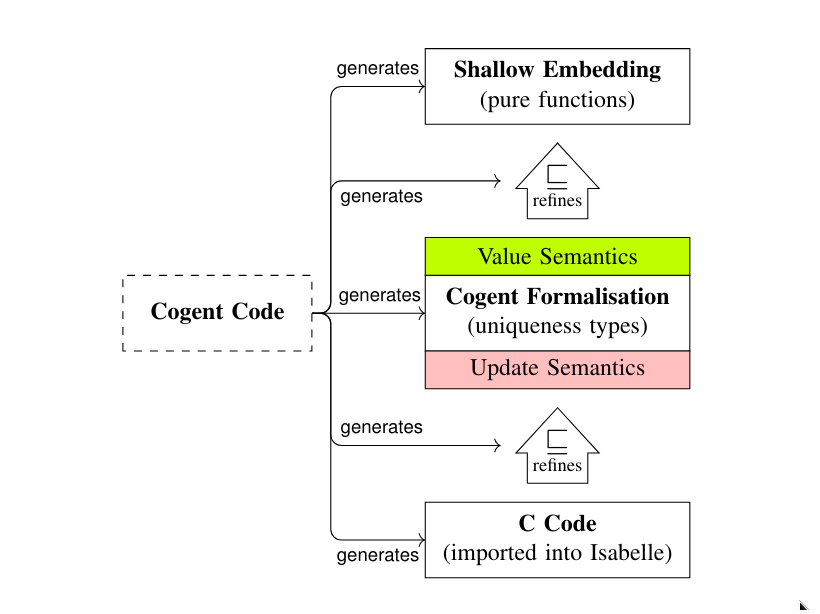
\includegraphics[width=0.85\textwidth]{figures/dargent_pipeline.png}
    \caption{The Cogent refinement framework (adapted from \cite{dargent_isola}). 
  Each box represents an embedding of the same Cogent program within Isabelle/HOL, 
  and arrows denote refinement proofs that establish semantic equivalence between 
  successive representations. 
  This verified foundation underpins later extensions such as Dargent, 
  which introduces declarative data-layout descriptions within the Cogent toolchain.}
    \label{fig:dargent_pipeline}
\end{figure}

\subsubsection{Extending the Lineage}
Earlier foundational work by \textbf{Tuch} (2008) formalized C's
pointer and heap semantics and Isabelle, laying the groundwork for verified
reasoning about memory at the byte level~\autocite{tuch2008formal}. More
recently, efforts such as a \textbf{Cornucopia} for CHERI
architectures~\autocite{filardo2020cornucopia} continue to
push forward verified compilation toward more realistic representations of
machine memory. 

Cedar builds directly on this insight. It seeks to extend the
extend the idea of \textbf{type-layout separation} and layout well-formedness
checking to the broader C ecosystem, without imposing
Cogent's functional restriction or proof obligations. In this sense, Cedar
generalized the principles pioneered by Dargent, bringing declarative layout
specifications to conventional systems programming. 

\subsection{Declarative and Domain-Specific Layout Languages}
While verified compilers focus on proving that compilers focus on
proving that compilation preserves meaning, a complementary tradition in
language design makes the data \textit{representation} explicit
through \textbf{declarative schema or layout languages}. These languages
allow programmers to describe binary formats at a high level, from which
parsers, serializers, and accessors, can be generated automatically.
Their goal is not proof of semantic equivalence, but \textbf{automation,
maintainability, and safety} in specifying
how structured data maps to bytes.

\subsubsection{Academic Layout Description Languages}
Early research systems such \textbf{PADS} and \textbf{DataScript} pioneered
declarative specifications of binary
data~\autocite{fisher2005pads,back2002datascript}. PADS introduced a system for
ad-hoc data formats, enabling automatic parser generation and providing
basic static checks such as field coverage
and alignment consistency. 
\textbf{DataScript}~\autocite{back2002datascript}, developed at Stanford,
treated binary layouts as first-class constructs: programmers defined bit-level
field structures and constraints, and the compiler generated Java classes to
read and write them. These languages were influential in showing that low-level
binary parsing could be expressed declaratively rather than through manual
bit-twiddling code. 

\subsubsection{Industrial Serialization Frameworks}
Many of these academic ideas re-emerged in modern industrial
frameworks designed for cross-platform serialization and
inter-process communication. Tools such as
\textbf{FlatBuffers}~\autocite{flat_buffers} and 
\textbf{Cap'n Proto}~\autocite{capn_proto_serialization}
use \textbf{interface definition languages} (IDLs) to describe data
schemas from which efficient, type-safe code is generated automatically.
These frameworks guarantee binary compatibility across architectures
and languages, reducing the likelihood of layout mismatches between
communicating components.

The \textbf{Cap'n Proto} and \textbf{FlatBuffers} tools focus on
zero-copy access: data can be read directly from the
serialized buffer without immediate unmarshalling. This design
aligns with the performance goals of systems programming but
constrains data access to API-generated methods
rather than arbitrary pointer arithmetic. A recent survey by
\textbf{Vioti and Kinderkhedia (2022)}  catalogues these binary specifications
and highlights trade-offs between expressiveness, schema evolution, and
safety~\autocite{viotti2022survey}. 

Recent work has begun on examining these tools from a \textbf{security
pers}. \textbf{Lilly Sell's (2024)} analyses the schema semantics of
FlatBuffers and its implementation to identify classes of layout
vulnerabilities and unsafe pointer usage~\autocite{sellsecurity}. The
study emphasizes that, despite their strong type systems, industrial
IDLs provide no formal guarantees about in-memory safety or field alignment
once data is accessed through unsafe code. These findings
underline that even modern frameworks remain
vulnerable when low-level layout details escape the boundaries of their
generated APIs.

\subsubsection{Comparing Declarative Layout Languages}
Declarative layout frameworks share several design principles:
\begin{enumerate}
    \item they separata \textit{logical structure} from\
    \textit{physical representation},
    \item they generate accessors and parsers automatically; and
    \item they provide at least partial checks for field consisteny or
    alignment.
\end{enumerate}

However, they typically operate in \textbf{controlled environments}—either
within managed runtimes or through generated API layers—and are not designed
for \textbf{arbitrary pointer-level operations} common in systems code.
Their safety guarantees therefore stop at the interface boundary: once raw
memory is accessed directly, correctness again depends on the programmer.

%Table of compariosn of DSL (PADSm DataScript, BinX, FlatBuffers, Cap'n Proto
%Avro and Cedar)

Cedar builds on this lineage by re-introducing declarative layout control
\textit{within C} itself. It inherits Dargent's separation between logical
physical layouts but targets a more permissive,
imperative environment. Where existing DSLs stop at schema generation,
Cedar amis to provide static well-formedness checking and direct compatibility
with verified C toolchains such as CompCert. In doing so, it connects the
two worlds of declarative layout description and
verified low-level systems programming. 

%FFigure of Declarative layout timeline
%PADS -> DataScript -> BINX -> Industrial IDLS -> Dargent -> Cedar

\subsection{Runtime Safety and Analysis Tools}
When low-level layout errors escape compile-time detection, developers rely on
\textbf{runtime instrumentation} and \textbf{static or dynamic analysis} to
locate faults.
These tools do not prevent misuse of memory, but they help identify common
classes of errors such as buffer overflows, uninitialized reads, and invalid
pointer dereferences.

\subsubsection{Dynamic Analysis Tools}
Dynmaic instrumentation frameworks such as
\textbf{Valgrind/Memcheck}~\autocite{valgrind} monitor every
memory access to detect invalid reads and writes at byte granularity.
Compiler-based sanitizers—including \textbf{AddressSanitizer (ASAN)},
\textbf{UndefinedBehaviorSanitizer (UBSAN)}, and
\textbf{MemorySanitizer (MSan)}—insert checks into generated code to catch
access errors and violations of the C standard at runtime~\autocite{ubsan,asan}.
These tools have been widely adopted in testing and continuous-integration
pipelines because they can reveal elusive bugs that arise from
undefined behavior, alignment faults,
and mis-computed offsets.

However, such techniques are inherently \textbf{reactive}. They only
detect errors along exercised execution paths and their effectiveness
depends heavily on the completeness of test coverage.
In addition, instrumentation typically incurs in non-trivial
runtime overhead—Valgrind can slow execution by an order of magnitude—making
these tools unsuitable for production or embedded environments. While
they are indispensable for debugging, they provide \textbf{no guarantee}
that untested code is free from layout mismatches or that binary
representations remain consistent across architectures. 

\subsubsection{Static Analysis and Type-Based Approaches}
Complementary static analyses attempt to infer
memory usage and pointer relationships directly from source code.
Tools such as \textbf{Cclyzer} perform
\textbf{points-to and structure-sensitive analysis} to detect potential
type violations~\autocite{balatsouras2016structure}. 
These methods can flag probable bugs before execution, but their
results depend on heuristics and may yield false positives or incomplete
coverage for low-level bit-manipulation code. Static analyses
are particularly challenged by C's weak type system and unrestricted
pointer arithmetic, which blur the boundary between logical structure
and physical representation.

\subsubsection{Safer Systems Languages}
Alongside external tools, modern systems languages incorporate
safety directly into their type systems. \textbf{Rust}, for
example, enforces memory safety through ownership and borrowing rules
that prevent data races and use-after-free errors at
compile time~\autocite{Rust_lang,Rust_systems}. Attributes
such as \texttt{\#\[repr(C)\]} allow Rust structures to
maintain binary compatibility with C while preserving the language
safety guarantees~\autocite{rust_repr}. However, Rust's model does not
eliminate layout variability entirely: padding and alignment remain 
platform-dependent, and many performance-critical routines still
resort to \texttt{unsafe} code when manipulating bit-fields or
packed data~\autocite{unsafe_rust}.

Emerging projects such as \textbf{Carbon} aim to modernize C++ while
improving safety and tooling~\autocite{carbon_cpp_safety}. Yet their
treatment of low-level representation is still evolving;
fine-grained layout control and verified layout correctness are not
current design goals.

These language-level solutions demonstrate the growing demand
for safer systems programming, but they also show
how difficult it is to combine \textbf{fine-grained control} with
\textbf{formal assurance}. Cedar occupies a complementary niche: it does
not replace C or enforce a new ownership mode, but instead
introduces \textbf{declarative layout specification} within existing
C codebases, addressing correctness at the representation layer. 

\subsubsection{Hardware-Assisted Memory Safety}
Recent research explores hardware extensions to enforce spatial and temporal
safety directly in the architecture. The \textbf{Capability Hardware
Enhanced RISC Instructions (CHERI)} architecture introduces
bounds and permissions to pointers, preventing many classes of buffer overflow
and use-after-free errors\autocite{filardo2020cornucopia}. Building on
this model, \textbf{Cornucopia} introduces efficient mechanisms for temporal
safety in CHERI heaps. Such approaches complement compiler instrumentation
by catching illegal accesses in hardware, greatly reducing overhead and enabling
fine-grained isolation between components.

Despite their effectiveness, these mechanisms do not reason about
\textbf{representation correctness}: they guarantee that accesses stay within
allocated bounds, not that the bytes being accessed correspond
to the intended logical structure. A program can be spatially safe
but still misinterpret a binary layout
if field offsets or bit-widths are wrong. Hardware capabilities thus solve
one aspect of memory safety—protecting allocation boundaries—while leaving
layout correctness to the programmer. 

\subsubsection{Positioning Cedar}
Runtime and static tools collectively enhance robustness but they remain
\textit{after-the-fact} defenses. They identify violations of memory
safety rather than enforcing \textit{design-time correctness} of layouts.
Cedar approaches the problem from the opposite direcion: by
\textbf{declaring layouts explicitly} and checking their compatibility
with corresponding C types before compilation, it aims
to prevent entire categories of representation errors that dynamic tools
can only detect later. Where Valgrind and sanitizers
ensure that a memory access is valid, Cedar, ensures that the 
access corresponds to the \textit{right bytes}. In this sense,
Cedar complements runtime verification and hardware enforcement, providing a
static foundation on which these broader safety mechanisms can rely.


\subsection{Summary and Research Gap}
This chapter has reviewed the landscape work related to data-layout
control and memory safety in systems programming. The discussion
began with the \textbf{C memory model}, where representation
details such as alignment, padding and field order remain
underspecified and vary across compilers and architectures.
These ambiguities complicate reasoning about correctness and performance in
context such as device drivers and protocol stacks. Subsequent
sections examined how \textbf{verified compilers} and \textbf{languages},
exemplified by CompCert, Cogent and Dargent, have provided rigorous guarantees
about program semantics and layout correctness—but only within constrained or
abstracted settings. Other efforts, from \textbf{declarative layout DSLs} like
PADS and DataScript, to \textbf{industrial frameworks} such as FFlatBuffers
or Cap'n Proto, have demonstrated that high-level schema descriptions
can improve maintainability and portability, albeit without
formal assurance for in-place C data structures. Finally, the chapter
considered \textbf{runtime tools, hardware capabilities}, and \textbf{safer
systems languages} such as Rust, which mitigate many classes of memory errors
but do not address the root of the problem of explicitly specifying and
verifying layout semantics.

Across these approaches, a consistent limitation emerges. Verified compilers
assume layouts are correct but cannot check them. Declarative frameworks desribe
layouts but operate outside the C toolchain. Runtime tools detect violations
only after execution. None provide a \textbf{language-integrated, static
guarantee} that a C data structure's physical representation corresponds to its
intended logical form.

\textbf{Cedar} aims to bridge this gap. It brings declarative layout
philosphy of Dargent into the C ecosystem, allowing programmers to define
and check binary layouts directly alongside
their types. By separating logical structure from physical representation,
performing static well-formedness checks and generating cohesive C artifacts,
Cedar seeks to make low-level layout design both
expressive and reliable. The next chapter presents the
\textbf{design methodology} and \textbf{systems architecture} underpinning
this approach, outline how Cedar's compiler pipeline and language
features were developed and evaluated. 
\section{Methodology and Implementation}
This chapter presents the design principles and implementation of
\textbf{Cedar}, a prototype language and compiler for describing
C layouts declaratively.
The goal of the project is to give programmers
\textbf{greater trust} that in-memory representations of data structures
corresponds to their intent.
Cedar achieves this bya introducing a small external language
for layout declarations, paired with a static checker that validates 
those declarations against C type definitions and generates
layout consistent C code.

While we previously reviewed related work, this chapter focuses on what
was built: the theoretical foundations on which Cedar stands, the kind
of layouts it supports, and the design of its grammar and compilation
pipeline.
The work draws on two main sources of inspiration—\textbf{CompCert} and
\textbf{Dargent}—whose ideas on form the conceptual basis for
Cedar's semantics and tooling.

\subsection{Foundations: CompCert and Dargent}
Cedar's design is built upon the semantic foundations provided by
\textbf{CompCert}~\cite{leroy2009formal}, and the declarative layout
principles introduced by \textbf{Dargent}~\cite{dargent}.
Understanding these two systems explains both the motivation
and structure of Cedar.

\subsubsection{CompCert verified C semantics as a foundation}
CompCert~\autocite{compcert} is a formally verified compiler of the C language
Its significance lies 
in \textbf{formal definition of the C memory model}~\autocite{leroy2012compcert},
which specified how C objects are represented as contiguous blocks of bytes,
how pointer arithmetic and aliasing work, and under what condition two
memory states can be considered equivalent.
Although Cedar is not yet built \textit{within} CompCert, it adopts
the same conceptual views on C memory: objects are typed, laid out in
addressable bytes, and subjected to well-defined alignment and
padding rules.

By grounding Cedar's reasoning in this model, layout checking can be 
interpreted consistently within verified C semantics.
For example, when Cedar computes bit-ranges, and checks for non-overlapping
fields, it effectively enforces that the resulting layout 
would be \textbf{well-formed under CompCerts memory abstraction}. The
connection ensures that, if Cedar layouts were eventually compiled through
CompCert, their structural assumptions would remain sound.

\subsubsection{Dargent: declarative layouts and type-layout separation}
While CompCert provides the semantic bedrock, Cedar's language design
follows the philosophy of \textbf{Dargent}~\autocite{dargent}.
Dargent introduced a declarative approach to specifying how algebraic data types
are represented in memory, separating the physical layout from the logical
structure.

Cedar adopts key ideas—\textbf{type-layout separation} and \textbf{explicit
field placement}—but targets them for plain C rather than Cogent. Unlike Dargent,
Cedar does not require a restricted functional language, or a theorem prover;
it provides lightweight static checking that enforces the same
well-formedness properties. These adaptations transform Dargent's research
concept into a more practical, C-oriented tool.

\subsubsection{Bridging the Two influences}
Cedar can thus be viewed as a \textbf{bridge between CompCert and Dargent}:
From CompCert, it inherits a precise understanding of how C objects
occupy memory; from Dargent, it inherits a declarative notation for describing
that occupation explicitly.
Cedar's goal is to close the gap between declarative layout specifications
in self-contained languages, and the C ecosystem, producing verifiable code
that remain compatible with existing C compilers.

The remainder of this chapter builds on these foundations.
We continue by describing the subset of C types supported by Cedar and how
layouts are represented. Later we detail the language patterns and features.
Finally, we summarize the compiler architecture that realizes it.

%Figure of Cedar's lineage
\subsection{Language Overview}
Cedar operates over a well-defined subset of the C type system that
reflect the representations defined by CompCert. The
prototype focuses on data structures whose layout is
statically determinable: \textbf{structures, arrays, and
tagged unions}. These cases cover the majority of layout-sensitive
code in low-level programming while remaining tractable for static
checking.

\subsubsection{Structures}
Cedar treats C \texttt{struct} as ordered collections of named
fields occupying contiguous regions of memory.
Each field has a known size and alignment derived from its
base type.
A layout declaration for a structure describes the physical
order and spacing of its fields using placement
directives
such as \texttt{at}, \texttt{before}, and \texttt{after}.
During checking, Cedar ensures that:
\begin{itemize}
    \item All fields of the corresponding C \texttt{struct}  are
    represented exactly once,
    \item No two fields overlap in their bit ranges, and
    \item The overall size and alignment conform to the
    base types requirements.
\end{itemize}

This model allows Cedar to detect and properly handle changes that could
otherwise be silently mishandled by compiler-specific padding or mis-ordered
field declarations—one of the most common causes of data-layout bugs in C.

\subsubsection{Arrays} 
Arrays are represented as repeated layouts of a uniform elemenet type.
Cedar supports both fixed-length and statically known arrays.
The layout checked verifies that the element layout
is well-formed and then replicates its size and alignment
across the declared array length.
Array support enables Cedar to express memory regions such as
device register tables, or network buffers that consist of repeated
records.

\subsubsection{Primitive and Derived Types}
Base types such as \texttt{char}, \texttt{short}, \texttt{int}, \texttt{long},
and their fixed-width equivalents (\texttt{int8\_t}, \texttt{uint32\_t}, etc.)
are treated as atomic elements with known bit sizes and alignment constraints.
Cedar assumes the same type sizes as the host compiler, which can be
configured when the tool is built.
Pointer types are recognized but not yet given explicit layouts;
they are treated as opaque machine words, leaving pointer
validity and aliasing to the underlying C semantics.
Future extensions could integrate CompCert's pointer-value
model to reason about pointer fields more precisely.

\subsubsection{Layout Representation}
Internally, every Cedar layout is reduced to a \textbf{set of
non-overlapping bit-ranges} withing a contiguous address space.
Each range corresponds to a field array element and is annotated with its
logical name, type, and alignment.
FIGURE illustrates this mapping for a simple \textttt{struct} example.

%TODO Figure of example
% layout Student at 0 {}
% name: char[32]
% id: uint43__t after name
% grade: uint8_t after id

The compiler computer explicit offsets—\texttt{name} [0-255],
\texttt{id} [256-287], \texttt{grade}[288-295]—and verifies
that these regions are contiguous and non-overlapping.

This representation follows the same notion of "memory chunk" used in CompCert,
where each object occupies a sequence of bytes and field addresses are
computed as offsets within that chunk.
By maintaining this correspondence, Cedar's checked
layouts can be compiled through any C toolchain, including CompCert,
without violating its memory-safe assumptions.

\subsubsection{Scope and Limitations}
The current prototype omits constructs whose semantics 
complicate static layout reasoning, such as: bitfields,
flexible array members, recursive layouts, and untagged unions.
These features will be considered in future work
once the core checking mechanisms are stable.
Despite these restrictions, the implemented subset is expressive
enough to capture common data representations used in
device drivers, network protocols, and binary file formats.

\subsection{Cedar Language Design and Core Features}
Cedar extends C with a minimal set of declarative constructs for specifying
how data structures are laid out in memory.
Its syntax follows C's lexical convnetions but introduces
new top-level \texttt{layout} blocks
that describe the physical
placement of fields.
These layouts declarations are currently written in separate
\texttt{.cedar} source file and linked to existing C type
definition.
The language is intentionally small: its expressiveness
comes from composable placement directives rather than
complex new forms.

\subsubsection{Core Grammar}
FIGURE summarizes the grammar of Cedar's core language, adapted from
Anderson's proposal~\autocite{cedar_george}.

%figure of the grammar George

Each \texttt{layout} declaration associates a name (matching a C type) with
a collection of fields. Each field declaration specifies the type and
placement of a field relative to the layout's origin
or to other fields.

The \texttt{placement} clause may be absolute (\texttt{\@}) or relative
(\texttt{before}/\texttt{after}).
Recursive or parametric layouts are excluded.

%Example of student layout
%layout Student = record {
%  name  : U8[32] @ 0B,
%  id    : U32    after name,
%  grade : U8     after id
%} @ 0B;

In this example, the \texttt{Student} layout begins at offset 0.
The field \texttt{name} is an array of 32 characters
occupying the first 256 bits; \texttt{id} is placed immediately
after it, and \texttt{grade} follows \texttt{id}.
Offsets are computed automatically during the layout-checking phase.
If two fields were to overlap, or if a field were missing compared
to the associated C type, the checked
would reject the layout.

%Figure annotated same example as above.

\subsubsection{Language Semantics}
Cedar's semantics are deliberately simple and static.
Each layout defines a total mapping from logical fields to \textbf{bit-ranges}
within a contiguous address space.
The compiler computes these ranges deterministically based on field
sizes and placement directives.

\textbf{Key properties enforced by the checked:}
\begin{itemize}
    \item \textbf{Completeness} — every field of the corresponding C type
    must appear in the layout.
    \item \textbf{Non-overlap} — no two fields occupy intersecting bit ranges 
    \item \textbf{Order Consistency} — relative directives (\texttt{before}/\texttt{after})
    must refer to existing fields.
    \item \textbf{Alignment} — offsets must respect the alignment constraints
    of their base types.
\end{itemize}

A layout satisfying these rules is \textit{well-formed}. The checking
algorithm ensures that every accepted layout could correspond to a valid C
memory representation.

\subsubsection{Design Considerations}
Cedar's syntax supports declarative rather than arithmetic.
Instead of writing numeric offsets directly, programmers may
express structural relationships—"\texttt{id} after \texttt{name}"—that
the compiler resolves into precise addresses.
This improves readability and reduces the risk of human error, while
still allowing absolute placement (\texttt{@}) when required
for interoperability with binary formats and hardware registers.

To keep the semantics tractable, Cedar omits features like computed
field expressions or conditional layouts.
The resulting language is small enough to reason about statically and
expressive enough to describe practical C structures.

\subsubsection{Supported Directives Summary}
\begin{center}
    \begin{tabular}{|| c c c||}
        \hline
        Directive & Purpose & Example \\ [0.5ex]
        \hline\hline
        \texttt{@} & Absolute placement.  & \texttt{id : u32 @ 64B;} \\
        \hline
        \texttt{after} & Place field immediately after another. & \texttt{grade : u8 after id;} \\
        \hline
        \texttt{before} & Place field immediately before another. & \texttt{prefix : u8 before name;} \\
        \hline
        \texttt{layout} & Define a new layout block. & \texttt{layout Student { ... }} \\
        \hline
    \end{tabular}
\end{center}

Together , the grammar and these directives define Cedar's core language.
They form the user-facing layer of the system which is then translated by
the compiler into a sequence of well-defined intermediate representations.
These representations capture progressively more information
about the layout, allowing the checked to validate and later generate code
for the specified structures.

\subsection{Compiler Architecture}
Cedar's compiler is organized as a sequence of \textbf{pure translation stages}
that progressively enrich the information available about each layout.
This implementation is lightweight and research-oriented.

%Figure about compiler flow

Each stage transforms the program into a slightly more concrete form,
preserving the structure while adding derived information such as absolute
offsets and alignment constraints.

\subsubsection{Parsing and Resolution}
The grammar is parsed into a structure abstract syntax tree (\texttt{L}).
A resolution pass then substitutes symbolic references (e.g., \texttt{after name})
with explicit dependencies between fields.
Each field returns its declared attributes—type, byte offset, relative placement,
and optional endianness.
At this point the layout is still declarative: field positions are
described relative to one another rather than as numeric offsets.

The parser currently supports: Nested constructs, quoted field names, and forward
references between fields. Comments and diagnostics, and multiple layouts per
field are not yet implemented. Parse errors are reported generically.

\subsubsection{Static Checking}
In the next stage (LR), the compiler resolves \textbf{relative placements} and
\textbf{nesting}. Every symbolic reference (\texttt{after x}, \texttt{before y})
is replaced with a concrete byte offset computed from previously defined fields.
Nested \texttt{record} blocks are \textbf{flattenned} into a single
linear sequence of fields using compound names (e.g., \texttt{grade_maths}).
Endianness and element size information are propagated through this transformation.

The resulting \textit{lowered representation (LR)} is a canonical, order-independent
list of fields, each with a fixed, offset, size and endianness tag.

The \textbf{checked representation (CR)}  introduces explicit byte ranges.
Offsets are multiplied by eight to produce bit ranges for each field, which
allow the code generator to reason about sub-word accessess and multi-word
values.
Cedar performs basic consistency checks during this phase:

\begin{itemize}
    \item fields do not overlap,
    \item offsets must be non-negative and monotonically increasing, and
    \item all fields must have defined sizes.
\end{itemize}

Full alignment checking, total-size verification, and overlap proofs are
not yet implemented, but the structure is designed to accommodate them later
\subsubsection{Code Generation}
The final stage translated the checked representation into compile-able C code.
The output consists of:
\begin{enumerate}
    \item A header file defining the a flat array of \texttt{uint32_t} words;
    and
    \item A C source file containing \textit{accessor} and \textit{mutator}
    functions for each field.
\end{enumerate}

Nested records are emitted as flattened field names; arrays are unrolled into
repeat accessors. Per-field endianness annotations are honoured by inserting
byte-swap operations in generated setters and getters.

No runtime support or special compiler modifications are required. The generated
code can be compiled by any C compiler, including \textbf{GCC} and \textbf{CompCert}.

\subsubsection{Design Rationale}
The architecture emphasizes two main principles:
\begin{enumerate}
    \item \textbf{Transparency}. Each representation (L, LR, CR) can
    be inspected, making the compiler's reasoning traceable
    \item \textbf{Modularity}. Additional analyses or transformations
    can be inserted between stages without disrupting others.
    \item \textbf{Extensibility}. The separation of passes makes it straightforward
    to extend the language (for example, by adding union layouts or precise bit-field control)
    without disrupting the core pipeline.
\end{enumerate}

This design allow Cedar to be extended in the future with
additional features, and potentially support for automated
verification, similar to Dargent.

It provides a practical foundation for Cedar's prototype: small enough
to experiment with, buth structured in a way that preserves the formal
clarity of its inspirations.

\subsection{Achievements and Scope}
The Cedar prototype demonstrated that declarative data-layout specification
can be integrated directly into the C programming environment in a practical
way.
Its development produced a complete end-to-end toolchain—from parsing and static
checking of layout descriptions to the generation of layout-consistent C
code—that validates the design concepts outlined in this chapter.

\subsubsection{Implemented Features}
The current implementation supports:

\begin{itemize}
    \item \textbf{Declarative layout defintions} for \texttt{structs},
    fixed-size arrays, and tagged unions.
    \item \textbf{Placement directives} (\texttt{at}, \texttt{before}, \texttt{after})
    that determine field ordering and spacing.
    \item \textbf{Automatic offset computation} and total-size calculation.
    \item \textbf{C code generation} producing equivalent declarations
    and accessor functions.
\end{itemize}

Each of these features we tested on representative examples derived from
Dargent's examples and from common systems-programming idioms such as
device registers. The prototype successfully detected layout mismatches
and generated compilable C code for all supported constructs.

\subsubsection{Scope and Limitations}
Cedar intentionally restricts its expressiveness to keep checking decidable
and the implementation lightwieght.
The prototype does \textbf{not} yet support:
\begin{itemize}
    \item Bit-fields or overlapping union members;
    \item Flexible array members or dynamically sized layouts;
    \item Nested or recursive layout definitions;
    \item Automated diagnostic recovery;
\end{itemize}

These omissions do not reflect missing functionality but a deliberate research
boundary: the implemented subset is sufficient to evaluate Cedar's design
principles and verify that they operate coherently within C's type system.
The language design and compiler architecture are modular enough that
these features could be added in future versions without
major restructuring.

\subsubsection{Practical Outcome}
The resulting system is a functioning compiler that demonstrates:
\begin{enumerate}
    \item Declarative layout syntax can describe C data structures succinctly;
    \item Static checking can verify structural inconsistencies that ordinary
    C compilers accept silently;
    \item Generated code remains portable and compatible with existing toolchains.
\end{enumerate}

Together, these results validate Cedar's underlying hypothesis: that
separating layout intent from C type declarations can improve
programmers' confidence in the correctness of low-level data representations.

The next chapter presents concrete example and results, illustrating how
Cedar's layout translate into verified C code and how its checker behaves
on representative cases.
\section{Implementation and Evaluation}
The previous chapter outlined the design principles and methodological
foundations guiding the development of Cedar. This chapter presents the
\textbf{realized prototype}, describing its implementation,
internal architecture, and preliminary evaluation. The aim is not to
demonstrate a production-ready compiler but to validate the design's
feasibility and examine how declarative layout specifications can
operate directly within the C ecosystem. The Cedar prototype serves as a
\textit{proof of concept} for the design-science process described earlier:
it embodies a set of language features and checking mechanisms from which
insights about expressiveness, soundness, and practicality can be drawn.

This chapter begins by providing an overview of the compiler's implementation
and module organization. It then delves into descriptions of
intermediate representations and key components—layout checking, type
matching, and code generation. Finally, it reports evaluation results
obtained form layout examples and reflects on design trade-ffs and lessons
learned.

\subsection{Language Syntax and Grammar}
Cedar extends the C programming language with a small set of
\textbf{declarative constructs} for describing how data is represented
in memory. Its syntax is intentionally compact and close to C, so that
programmers can reason about physical layout without leaving 
the familiar idioms of systems programming. A Cedar source file
defines one or more \textbf{layout declaration} that specify
the mapping between a logical C type and its concrete in-memory
representation. Each layout is associated with a base C type and describes
the placement, alignment, and size of its fields using a combination
of absolute and relative directives.

\subsubsection{Core Syntax}
%Figure
This grammar captures only the layout-level constructs; standard C syntax
for type declarations is assumed to exists
in companion \texttt{.h} or \texttt{.c} files. Layout declarations may
appear in any order, and can reference previously defined layouts through
identifiers.

\subsubsection{Example}
%code snippet
This example declares a memory layout for the \texttt{Student} structure.
The layout begins at bit offset 0.
Each field specifies a C type and a placement directive:
\begin{itemize}
    \item \texttt{name} is a fixed-size character array occupying the first 256 bits.
    \item \texttt{id} is placed immediately \textit{after} \texttt{name}, inheriting its offset plus size.
    \item \texttt{grade} follows \texttt{id}.
\end{itemize}

Cedar's compiler resolves these relationships to compute
explicit bit-ranges and verify that fields neither overlap nor exceed
the enclosing structure's bounds.

\subsubsection{Design Rationale}
The syntax follows three guiding principles:
\begin{enumerate}
    \item  \textbf{Familiarity:} preserve C's lexical style so existing 
    programmers can adopt Cedar easily.
    \item \textbf{Clarity:} keep layouts readable by expressing relationships
    (\texttt{after}, \texttt{before}) rather than numeric offsets.
    \item \textbf{Analyze-ability:} restrict constructs to a small, statically
    checkable core that can be reasoned about formally in future work.
\end{enumerate}
The existing prototype currently omits recursive and parametric layouts,
focusing on straightforward records and arrays. These restrictions simplify
reasoning about offsets and enable predictable code generation. Later
chapters discuss how these constructs translate through
the compiler pipeline and
into generated C code.

%Figure on how a layout is transofrmed into intermediate representations
% and finally C code.


\subsection{Implementation Overview}
Cedar has been implemented as \textbf{modular Haskell compiler}. 
The implementation follows a multi-stage architecture. 

%Figure illustrating the flow of the compiler

\subsubsection{Structure and Tooling}
The compiler is organized into clearly separated modules:

\begin{center}
\begin{tabular}{||c c ||}
    \hline
    \textbf{Module} & \textbf{Responsibility} \\ [0.5 ex] 
    \hline\hline
    \texttt{Surface.hs} & Defines the abstract syntax for user-facing Cedar constructs. \\
    \hline
    \texttt{Lexer.x and Parser.y} & Tokenize and parse \texttt{.cedar} files. \\
    \hline
\end{tabular}
\end{center}

\section{Future Work}
Although the examples shown show how valuable a tool like
Cedar can be, it also highlights several avenues for future development.

\subsection{Language and Compiler Features}
There are a few features that were considered
out of scope for this initial implementation, however
they heavily limited the real world examples that could be tested
with Cedar. Implementing these features would greatly increase
the usefulness of the language and set it up as a tool useful
for real world systems programming and research.

\begin{enumerate}
    \item Complete well-formedness checking: The current implementation
    does not perform a full static analysis of the layout.
    Implementing this should be a priority, and the current design
    leaves space for this to be added in future work. The CR stage
    calculates offsets and sizes required for this check to to take
    place, but it is not yet implemented.
    \item Missing Structures: Bit fields, unions and pointers
    are commonly found structures in C programs, and their support
    would immediately increase the amount of layouts that could be expressed
    with the language.
    \item Unified Array accessors: A trivial but useful addition
    would be to ensure the codegen stage generates a unified
    accessor for a whole array, as well as per-element accessors. 
    This would reduce the amount of glue code required to
    integrate Cedar intro existing C codebases.
\end{enumerate}

\subsection{Towards a Verified System}
As with its predecessors, Cedar was conceived as an idea
for a verified system for data-layouts.
The design of the language reflects this, and undertaking
the task of ensuring each of the internal translations
stages are formally verified, would be the first step into
turning Cedar into a verified tool that can integrate easily
with verified compilers such as CompCert in order to provide
end-to-end guarantees about code behavior.

\textbf{Formalizing Internal Representations}:

Each translation stage (L, LR and CR) encodes
a refinement of information. From a 
symbolic structure, to resolved offsets and finally concrete
bit ranges.
These transformations are functional and self-contained, enabling
automated reasoning about their correctness with a proof assistant such
as Roq/Coq.
Formalizing their behavior would enable proofs that layout meaning
is preserved across stages: that the semantics of a record array
in L correspond exactly to its bit-range representation in CR.
Such results would elevate Cedar into a verifiable component
with a broader compilation framework.

\textbf{Integrating with Verified Compilation}:

An interesting direction would be to develop a custom C compiler,
most likely adapting CompCert as it already provides a verified
pipeline, and integrate the Cedar compiler into that pipeline.
This would allow for Cedar code to be written in-line along with 
C code, creating a seamless experience for programmers who
need a fully verified toolchain for systems programming.

\textbf{Tooling visualization}:

As Cedar's analysis grows more sophisticated, corresponding improvements
in usability will become essential. Interactive visualization of layouts,
showing byte ranges, field names and endianness, could transform the compiler
into a teaching and debugging aid. 


% -------------------------------
% References
% -------------------------------
\printbibliography

% Appendices if you have them (keep your own files/structure)
% \appendix
% \section*{Appendix}
% \addcontentsline{toc}{section}{Appendix}
% \input{sections/appendix.tex}

\end{document}
